\documentclass{article}

% if you need to pass options to natbib, use, e.g.:
%     \PassOptionsToPackage{numbers, compress}{natbib}
% before loading neurips_2024


% ready for submission
%\usepackage{neurips_2024}


% to compile a preprint version, e.g., for submission to arXiv, add add the
% [preprint] option:
%\usepackage{neurips_2024}


% to compile a camera-ready version, add the [final] option, e.g.:
\usepackage[final]{neurips_2024}
\usepackage{graphicx}
\usepackage[most]{tcolorbox}     % 支持 breakable + listing
\tcbuselibrary{listings, skins}  % 如果想语法高亮
\tcbuselibrary{skins, breakable}

\usepackage[linesnumbered,ruled,vlined,noend]{algorithm2e}


% to avoid loading the natbib package, add option nonatbib
%\usepackage[nonatbib]{neurips_2024}


\usepackage[utf8]{inputenc} % allow utf-8 input
\usepackage[T1]{fontenc}    % use 8-bit T1 fonts
\usepackage{hyperref}       % hyperlinks
\usepackage{url}            % simple URL typesetting
\usepackage{booktabs}       % professional-quality tables
\usepackage{amsfonts}       % blackboard math symbols
\usepackage{nicefrac}       % compact symbols for 1/2, etc.
\usepackage{microtype}      % microtypography
\usepackage{xcolor}         % colors
\usepackage{amsmath}
\usepackage{siunitx}

\usepackage{tikz}
\usetikzlibrary{arrows.meta, calc, positioning, shapes.misc, matrix, graphs}

\usepackage{biblatex}
\addbibresource{ref.bib}
\title{
    \Large Train Large Models Across the World: Accelerating Training on Geo-Distributed Heterogeneous Clusters
    via \emph{Subservers} and Bandwidth-Aware Collective Communication\\[1em]
    \normalsize CS650 Project Final Report
}

\usepackage{algorithm}
\usepackage{algorithmic}
\usepackage{caption}

% The \author macro works with any number of authors. There are two commands
% used to separate the names and addresses of multiple authors: \And and \AND.
%
% Using \And between authors leaves it to LaTeX to determine where to break the
% lines. Using \AND forces a line break at that point. So, if LaTeX puts 3 of 4
% authors names on the first line, and the last on the second line, try using
% \AND instead of \And before the third author name.


\author{%
  Yuxiang Lin \\
  %Department of Computer Science\\
  %Cranberry-Lemon University\\
  %Pittsburgh, PA 15213 \\
  %\texttt{hippo@cs.cranberry-lemon.edu} \\
  % examples of more authors
  \And
  Tianjun Yuan \\
  %Affiliation \\
  %Address \\
  %\texttt{email} \\
  % \AND
  % Coauthor \\
  % Affiliation \\
  % Address \\
  % \texttt{email} \\
  % \And
  % Coauthor \\
  % Affiliation \\
  % Address \\
  % \texttt{email} \\
  % \And
  % Coauthor \\
  % Affiliation \\
  % Address \\
  % \texttt{email} \\
}


\begin{document}


\maketitle


\begin{abstract}
Next‑generation foundation models are expected to break the \SI{100}{T}‑parameter
barrier, demanding over $10^{25}$\,FLOPs—well beyond the power and network
limits of any single GPU cluster.
We argue that \emph{geo‑distributed} training will be required.
With a real-world cluster distribution consideration, we introduce the \textbf{subserver} topology:
each metropolitan cluster talks to a nearby \emph{subserver} over a
multi‑terabit bandwidth Internet link,  while subservers exchange
gradients and activations.
We develop a two‑tier cost model that
(1)~chooses pipeline stages across subservers and
(2)~mixes data \emph{and} tensor sharding inside every cluster,
analysing the trade‑off.
We further apply a full OMNeT++ simulation on eight AWS regions with several clusters in each region.
\end{abstract}

\section{Introduction}

Training large language models has outgrown the capabilities of a single server, prompting a shift towards collaborative training across multiple datacenters. According to scaling laws, the next generation of frontier models may require hundreds of trillions of parameters \cite{gherghescu2024look}. Even hyperscale infrastructures with \SI{10}{\micro\second} switch latencies are constrained by limits on power, cooling, and fiber optics, making it infeasible to host such vast models within a single metropolitan area.

We propose a subserver-centric training framework that adapts the parallelism strategy to each level of a heterogeneous, geo-distributed network. Specifically, we adopt:
\begin{itemize}
\item Pipeline parallelism across subservers,

\item Data and tensor parallelism within each metro area to fully utilize high-bandwidth fabrics such as Jupiter.
\end{itemize}

Using a compact $\alpha$–$\beta$ communication model, we demonstrate conditions under which the added cost of local collective operations in tensor sharding is outweighed by the reduction in global communication time.

\paragraph*{Contributions.} \begin{itemize}\setlength\itemsep{0.2em} \item \textbf{Subserver topology:} A practical relay-layer architecture that efficiently aggregates metro-area traffic. \item \textbf{Unified scheduling model:} A parallelism-aware scheduler that jointly optimizes pipeline, data, and tensor strategies across heterogeneous clusters. \item \textbf{Tensor parallelism trade-off analysis:} A closed-form bound to determine whether sharding model weights leads to faster training for a given layer or parameter configuration. \item \textbf{End-to-end simulation:} An OMNeT++-based prototype simulating geo-distributed training across eight AWS regions, each containing multiple compute clusters. \end{itemize}



\section{Background and Motivation}

% \subsection{Heterogeneous Network}

% A network of nodes can be represented by a directed graph, where the vertices correspond to the nodes. There exists a directed edge $e$ between every pair of vertices with an associated edge cost $(\alpha_e, \beta_e)$ representing a link between two nodes. The $\alpha$-$\beta$ model \cite{hockney1994communication} represents the latency with $\alpha$ and reciprocal bandwidth with $\beta$, such that the cost of sending a chunk of size $n$ through the link takes time $\alpha + \beta n$.

% Our setting builds on these ideas by designing a \emph{virtual topology} simulating a world map. Close geographic points form clusters, each containing one or more \emph{subservers} with high-bandwidth links for inter-regional data exchange. In this way, each client in a cluster has fast local access to its subserver, while subservers collectively support efficient cross-region communication—an architecture that aims to reduce latency and overhead for distributed training at scale.

\subsection{Collective Communication Primitives \& Parallelism Taxonomy}

\textbf{Concepts.}  Large‑batch SGD relies on three bandwidth‑hungry collectives:  

(i) \emph{ReduceScatter} splits a tensor across $P$ ranks and simultaneously sums corresponding slices

(ii) \emph{AllGather} concatenates those slices so every rank recovers the full tensor 

(iii) \emph{AllReduce} is simply a ReduceScatter followed by an AllGather.  

On top of these kernels, four orthogonal forms of parallelism are routinely combined to scale a deep network \cite{scaling-book}: 
\begin{itemize}
\item{\textbf{Data parallelism}}: replicate parameters, shard the mini‑batch,  
\item{\textbf{Fully‑sharded data parallelism}}: shard both activations and weights,  
\item{\textbf{Tensor/model parallelism}}: partition large weight matrices within a layer,
\item{\textbf{Pipeline parallelism}}: place consecutive layer groups on different devices.  
\end{itemize}
Hybrid schemes such as HDP/HPP \cite{ye2024asteroid} or SDPipe’s grid layout \cite{miao2023sdpipe} exploit a subset of these axes but typically ignore WAN latency and heterogeneous link rates \cite{luo2022efficient}.


\subsection{Decentralized Large Model Training}

With the rapid growth in the size of foundation models \cite{achiam2023gpt, touvron2023llama}, training large-scale neural networks on a single machine has become increasingly impractical. \emph{Distributed learning} \cite{chen2021distributed} tackles this challenge by splitting the computational and data loads across multiple nodes, alleviating resource bottlenecks. Modern large-scale training clusters are often heterogeneous, comprising CPUs, GPUs, and specialized accelerators \cite{duan2024efficient}.

However, looking ahead, scaling laws and recent capacity studies indicate that the next generation of foundation models may reach {\raise.17ex\hbox{$\scriptstyle\sim$}}100 T parameters—much larger than today’s GPT‑4‑class systems \cite{gherghescu2024look, achiam2023gpt}. Training such a model would demand on the order of $10^{25}$ FLOPs and sustained multi‑gigawatt power draw, far beyond the logistical limits of any single metropolitan region \cite{gherghescu2024look}. To unlock this level of compute, we advocate \emph{geo‑distributed} training that federates clusters on different continents, effectively creating a “planet‑scale” accelerator fabric whose aggregate capacity can absorb the required workload \cite{yuan2022decentralized}. 

\textbf{Internet speed and latency} also plays a significant role in \emph{geo‑distributed} training. Hyperscalers have begun to deploy RDMA‑over‑Ethernet (RoCE v2) backbones that interconnect \emph{tens of thousands} of GPUs with ${<}10\mu$s hop latency, demonstrated in Meta’s 2024 clusters \cite{romanow2003overview, gangidi2024rdma}. Upcoming photonic interposers such as Lightmatter’s \emph{Passage} also promise 10–100$\times$ higher bandwidth at a fraction of the power, enabling million‑GPU topologies \cite{chen2019graphene}. Moreover, algorithms like \emph{NetStorm} dynamically reconfigure gradient‑exchange trees to exploit heterogeneous, fluctuating wide‑area links, achieving up to $9\times$ speed‑ups over conventional parameter servers \cite{li2024accelerating}.
Taken together, these trends point to a near‑future in which multi‑gigabit transoceanic links, elastic optical fabrics, and adaptive communication schedules converge, allowing synchronized SGD across continents and, ultimately, the training of 'hundred times' models on a truly global pool of computation.


\subsection{Decentralized Training with \emph{Subservers}}

\begin{figure}[htbp]
    \centering
    \begin{minipage}[t]{0.48\textwidth}
        \centering
        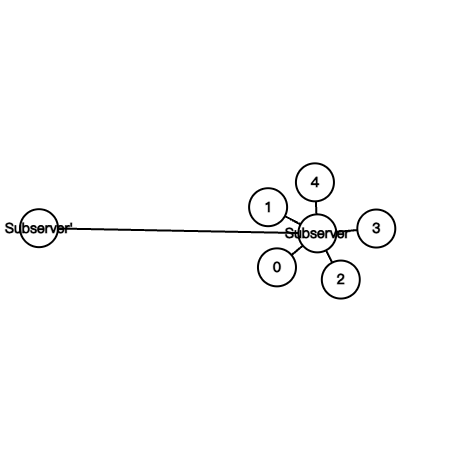
\includegraphics[height=0.2\textheight, trim=0 150 50 50,clip]{fig/subserver.png}
        \caption{Topology with \emph{Subserver}}
        \label{fig:subserver}
    \end{minipage}%
    \hfill
    \begin{minipage}[t]{0.48\textwidth}
        \centering
        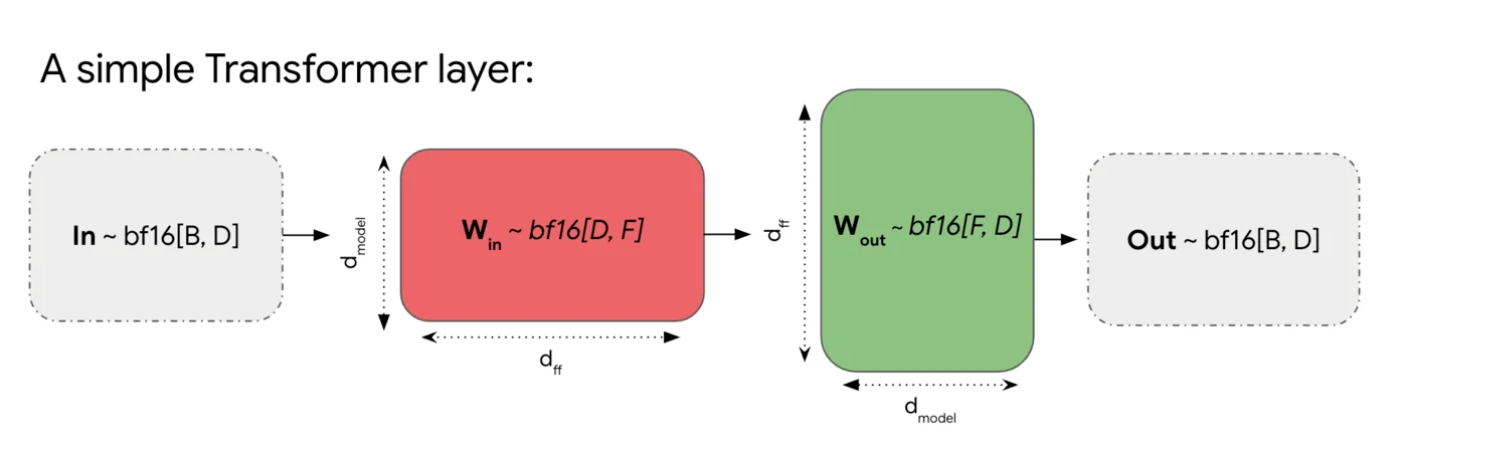
\includegraphics[width=\linewidth]{fig/simple.png}
        \caption{A Transformer layer simplified to two matrix multiplications \protect\cite[Part 5]{scaling-book}.}
        \label{fig:simple}
    \end{minipage}
\end{figure}


{\bf Urban clusters \& regional hubs.}  
Empirically, metro‑area “GPU cities’’ already exhibit {\raise.17ex\hbox{$\scriptstyle<$}}\SI{150}{\micro\second} round‑trip RTT between hosts—e.g.\ Google Cloud’s own intra‑zone measurements report a {\raise.17ex\hbox{$\scriptstyle\sim$}}\SI{66}{\micro\second} mean latency on 100 GbE links.  Inside such a area, fifth‑generation Jupiter fabrics now deliver up to \SI{13}{Pbit/s} of bisection bandwidth, implying per‑rack aggregates well above \SI{5}{Tbit/s} \cite{google_jupiter_2024}.

By contrast, distances between major cities stretch thousands of kilometres; end‑to‑end RTTs still range from {\raise.17ex\hbox{$\scriptstyle\sim$}}\SIrange{10}{60}{\milli\second} within continents and hover around \SI{60}{\milli\second} across the Planet \cite{equinix_latency_2023}. 

This issue in both \emph{bandwidth} and \emph{latency} motivates the introduction of a regional \textbf{subserver} that aggregates all local traffic and pipelines to a regional center (Fig.\,\ref{fig:subserver}).

\medskip
{\bf Link heterogeneity in the subserver topology.}  
\begin{itemize}\setlength\itemsep{0.3em}
    \item \textbf{Cluster $\to$ Subserver}: multi‑Terabit electrical or short‑reach optical fabric, RTT $\le\SI{0.15}{ms}$
    \item \textbf{Subserver $\leftrightarrow$ Subserver} (“metro $\leftrightarrow$ metro’’): long‑haul coherent optics at 400–800 Gb/s per lambda, RTT $\approx$\SIrange{10}{60}{ms}.  However, large bandwidth between Subserver significantly helps with our data trasmitting.
\end{itemize}




% \subsection{Collective Communication}

% \textbf{TODO: Introduce AllReduce, ReduceScatter, AllGather}


% \subsection{Parallel Large Model Training Techniques}

% We will explore the following ways to parallelize a DNN and the combination of these methods \cite{scaling-book}:

% \begin{enumerate}
%     \item \textbf{Data parallelism}: Activations sharded along $B$.
%     \item \textbf{Fully-sharded data parallelism}: Activations sharded along $B$ and parameters sharded along an axis.
%     \item \textbf{Tensor parallelism}: Parameters sharded along $F$.
%     \item \textbf{Pipeline parallelism}: Layers in the DNN pipeline sharded onto different devices.
% \end{enumerate}

% Current distributed ML approaches typically combine data and pipeline parallelism. The Asteroid paper \cite{ye2024asteroid} compares hybrid data parallelism (HDP) and hybrid pipeline parallelism (HPP), opting for HPP. HDP groups nodes, applying pipeline parallelism within groups and data parallelism between them, whereas HPP does the opposite. SDPipe \cite{miao2023sdpipe} organizes workers in a grid, using data parallelism along one axis and pipeline parallelism along the other.

% To optimize node assignment in pipeline parallelism, we build on the dynamic programming method from \cite{luo2022efficient}, also used in Asteroid \cite{ye2024asteroid}. Notably, \cite{luo2022efficient} ignores network latency and assumes AllReduce time is dictated by the lowest link bandwidth--assumptions unlikely to hold in heterogeneous networks like the Internet.

% We remark that unlike the data parallelism mentioned earlier, data parallelism in these works does not synchronize gradients every backward pass; instead, gradients remain sharded across batches and are periodically averaged.

% Unlike prior work, we explore all four types of model parallelism and their combinations, rather than limiting ourselves to data and pipeline parallelism.

% \begin{itemize}
%     \item \textbf{Data Parallelism}: The model is replicated across multiple devices, and each device processes a different mini-batch of input data. 
    
%     \item \textbf{Pipeline Parallelism}: The model is split into multiple layers, each assigned to a different device.
    
%     \item \textbf{\textcolor{blue}{Tensor Parallelism (What they haven't done)}}: Individual model layers are partitioned across devices at the tensor level. Each device computes a slice of the tensor.
% \end{itemize}


% Collective communication routines (e.g., AllReduce, AllGather) facilitate node communication during DNN training. We aim to design and implement routines that adapt to heterogeneous network topologies \cite{won2024tacos, cho2019blueconnect}.

% TACOS \cite{won2024tacos} generates topology-aware collective algorithms by modeling optimization as a link-chunk matching problem in a time-expanded network. While it supports heterogeneous networks via the $\alpha$-$\beta$ model, it assumes a uniform chunk size $n$ across all links. Though evaluated on heterogeneous topologies like 2D Switch, its link characteristics are drawn from a limited set, unlike the diverse conditions in Internet-connected nodes. Other automatic synthesis methods are even more constrained—TACCL \cite{shah2023taccl} only models symmetric node connections, while Blink \cite{wang2020blink} applies solely to one-to-many collectives.

% We plan to develop adaptive collective communication routines, building on TACOS \cite{won2024tacos}.

% \section{Motivation}

% With the rapid growth in the size of foundation models \cite{achiam2023gpt, touvron2023llama}, training large-scale neural networks on a single machine has become increasingly impractical. \emph{Distributed learning} \cite{chen2021distributed} tackles this challenge by splitting the computational and data loads across multiple nodes, alleviating resource bottlenecks. Modern large-scale training clusters are often heterogeneous, comprising CPUs, GPUs, and specialized accelerators \cite{duan2024efficient}; although such diversity can boost performance, it also complicates workload balancing and inter-node communication—particularly for collective operations like AllReduce and ReduceScatter \cite{won2024tacos, cho2019blueconnect} that aggregate gradients from all nodes. 

\section{Problem Formulation}

\subsection{Simplified Layer and Cost Model}

We model each Transformer block as two dense matmuls:
$\text{In}[B,D]\,{=}\,X\;
\stackrel{\cdot}{\rightarrow}\;
W_{\text{in}}[D,F]\;
\stackrel{\cdot}{\rightarrow}\;
W_{\text{out}}[F,D]$
(Fig.~\ref{fig:simple}).  Element‑wise ops are ignored because their cost is small compared with the $\Theta(BD^{2})$ multiplies.

Communication follows the $\alpha$–$\beta$ rule: sending $n$ bytes costs
$\alpha + \beta n$.  
Local links share $(\alpha_{\text{loc}},\beta_{\text{loc}})$,
while long‑haul links between Subservers share
$(\alpha_{\text{wan}},\beta_{\text{wan}})$ with
$\alpha_{\text{wan}}\!\gg\!\alpha_{\text{loc}}$.
Compute and communication overlap whenever their critical paths do not clash.
Our objective is to pick a parallelism plan that minimises the end‑to‑end
makespan on this two‑tier network.



\subsection{Parallelism on the Subserver Topology}

\begin{itemize}\setlength\itemsep{0.3em}
  \item \textbf{Subserver \& Subserver} (\SI{10} to \SI{60}{ms} RTT):  
        use \emph{pipeline parallelism}.  
        Each stage streams activations forward and gradients back,
        hiding most link latency behind compute
        \cite{huang2019gpipe, narayanan2019pipedream}.  

  \item \textbf{Cluster \& Subserver} ($\le\!\SI{0.15}{ms}$ RTT):  
        combine \emph{data parallelism} (split the mini‑batch) and
        \emph{tensor/model parallelism} (shard weight matrices).
        Fast fabrics make collectives such as \texttt{AllReduce} negligible
        \cite{shoeybi2019megatron, roberts2023scaling}.
\end{itemize}

Streaming coarse blocks over slow links and keeping fine‑grained synchronous
work inside fast links yields better utilisation than relying on any single
parallelism mode end‑to‑end.


% \textbf{(Describe distributed training over the Internet)}

% \subsection{Topology}

% \textbf{TODO: Note how we implement AllReduce (clients send to subserver, then subserver sends back to clients)}

% \textbf{(Describe geo-distributed clusters and subservers)}

\section{Analysis of Parallelism Approaches}

\subsection{Notations}

\begin{figure}[htbp]
    \centering
    \begin{minipage}[t]{0.48\textwidth}
        \centering
        \small
        \begin{tabular}{l|l}
            \textbf{Symbol} & \textbf{Meaning} \\
            \hline
            $L$ & Number of layers in the model \\
            \hline
            $D$ & $d_{\text{model}}$ (hidden dimension) \\
            \hline
            $F$ & $d_{\text{ff}}$ (feed-forward dimension) \\
            \hline
            $B$ & micro-batch size \\
            \hline
            $n, m_i$ & $n$ clusters, $i$-th cluster has $m_i$ clients \\
            \hline
            $i, j$ & The $j$-th client in $i$-th cluster \\
            \hline
            $b_{i, j}$ & Per-device micro-batch size \\
            \hline
            $(u), (d)$ & Upload/download \\
            \hline
            $c_{i, j}$ & Compute FLOPS \\
            \hline
            $v_{i, j}, w_{i, j}$ & Intra-cluster link latency and bandwidth \\
            \hline
            $V_{i_1, i_2}, W_{i_1, i_2}$ & Inter-cluster link latency and bandwidth \\
        \end{tabular}
        \caption{A table of symbols used and their meanings.}
        \label{tab:symbols}
    \end{minipage}%
    \hfill
    \begin{minipage}[t]{0.4\textwidth}
        \centering
        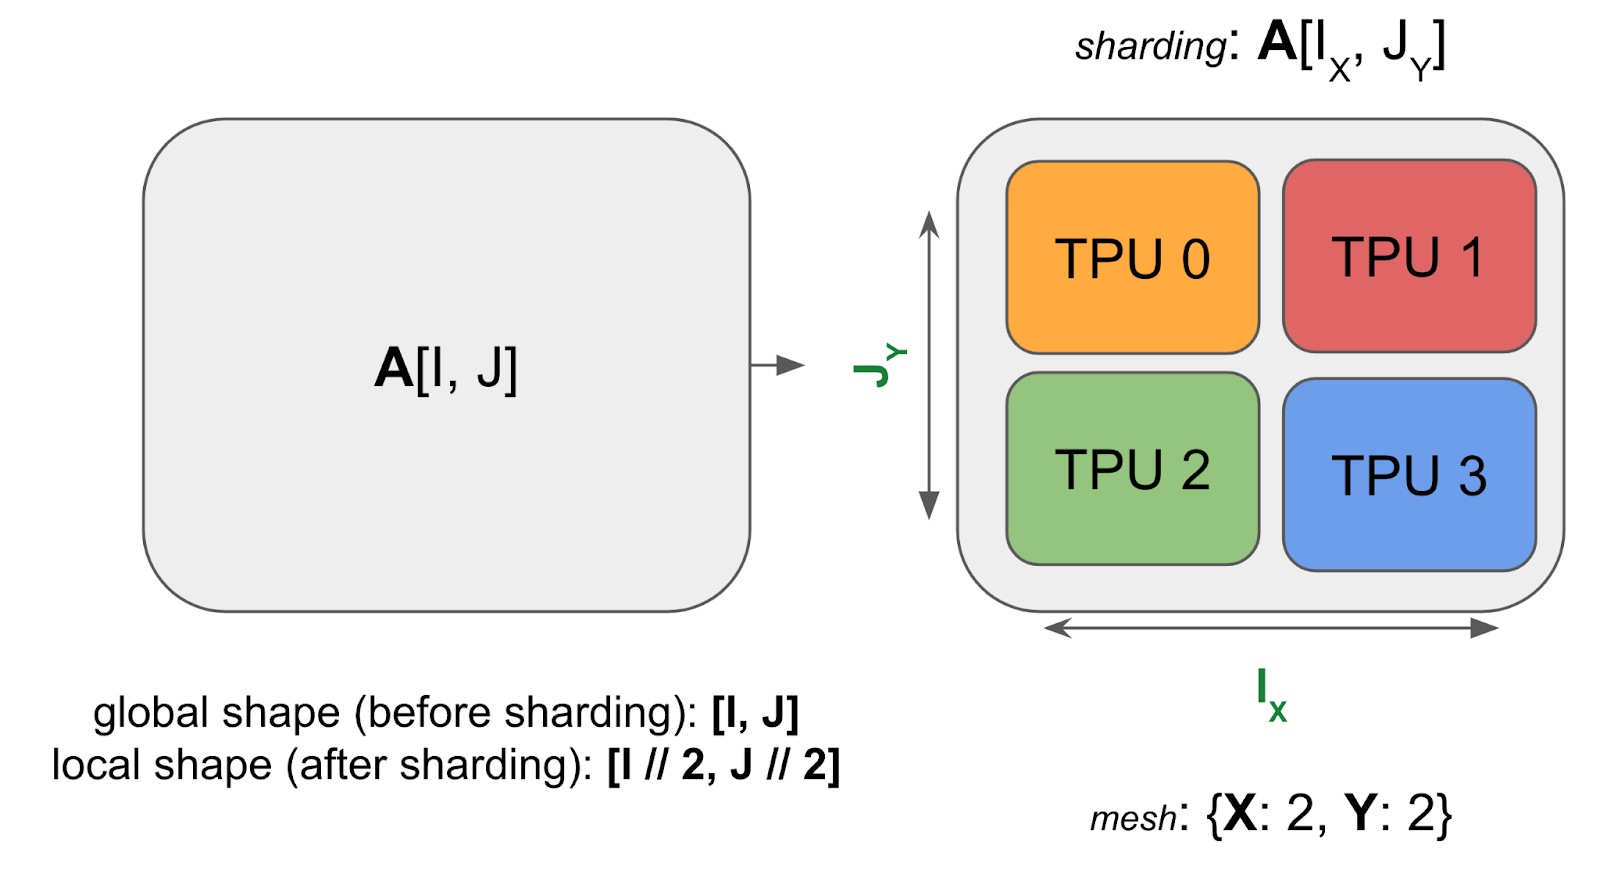
\includegraphics[width=0.95\linewidth]{fig/sharding.png}
        \caption{Sharding the tensor $A$ of size $I \times J$ over the $X$ and $Y$ axes respectively. Each device (TPU in this example) holds a piece of the sharded tensor.}
        \label{fig:sharding}
    \end{minipage}
\end{figure}


We use the same notation as in \cite[Part 3]{scaling-book} to represent a sharded tensor, which is a tensor divided along some axes and distributed among devices. $A[I, J]$ represents a tensor of size $I \times J$. $A[I_X, J_Y]$ is $A$ with $I$-dimension sharded along the $X$-axis, and $J$-dimension sharded along the $Y$-axis.

When multiplying two matrices along the same sharded axis in parallel, the results distributed among the devices need to be summed to get the final result. The summing operation is an AllReduce, which could also be decomposed into a ReduceScatter followed by an AllGather. For example:
\begin{align*}
    A[I, J_X] \cdot_J B[J_X, K] &\to C[I, K]\{U_X\} \\
    \text{AllReduce}_{X} C[I, K] &\to C[I, K] \\
    \text{ReduceScatter}_{X, K} C[I, K]\{U_X\} &\to C[I, K_X] \\
    \text{AllGather}_X C[I, K_X] &\to C[I, K]
\end{align*}

\subsection{Pipeline Parallelism}

Pipeline parallelism splits model layers across devices. It is useful for overcoming the memory constraint of individual devices and it is less communication intensive than the other parallelism approaches.

To prevent pipeline bubbles when using pipeline parallelism, multiple ``micro-batches" are sent down the pipeline before gradient update for the first micro-batch returns to the first layer. This will have a small negative impact on convergence due to using stale values. However, since we are unable to find a paper with analytical bounds for convergence when using micro-batching, we would assume that our approach would have a rate of convergence close to similar approaches such as \cite{ye2024asteroid}.

In our approach, pipeline parallelism is used across clusters, as the less communication intensive nature of pipeline parallelism is suitable for the high latency, high bandwidth links between the clusters. It also addresses the heterogeneity of memory resources among clusters by assigning more model layers to clusters with larger memory. However, this paper does not focus its analysis on the memory constraints.

Let $\pi_n$ be a permutation of $\{1, 2, \dots, n\}$, the inter-cluster communication cost without consider pipelining is
\begin{align}
    \sum_{i=1}^{n-1} \left(V_{\pi_{i}, \pi_{i + 1}} + \frac{BD}{W_{\pi_{i}, \pi_{i + 1}}}\right).
\end{align}

It is difficult to formulate the speedup caused by pipelining since the micro-batches approach each cluster at different times. Additionally, a different number of layers may be assigned to each cluster. However, suppose that the number of micro-batches is high, and that the layers are evenly assigned, the speedup of $n$ clusters in a pipeline can be approximated as a factor of $n$.

\subsection{Data Parallelism}

\textbf{Sharding Scheme:}
\begin{align*}
    \text{In}[B_X, D] \cdot_D W_{\text{in}} [D, F] \cdot_F W_{\text{out}} [F, D] \to \text{Out}[B_X, D]
\end{align*}

\begin{figure}
\centering
\resizebox{0.6\textwidth}{!}{%
\begin{tikzpicture}[
  node distance=1cm and 1cm,
  every node/.style={draw, minimum width=2cm, minimum height=1cm, font=\footnotesize, align=center},
  op/.style={circle, draw, minimum size=0.8cm},
  dashedop/.style={draw, dashed, minimum size=0.8cm, font=\footnotesize\itshape},
  ->, >=Stealth
]

% Top nodes
\node (dout) {dOut[\(B_X, D\)]};
\node[op, below right=of dout] (mul1) {\(\cdot_B\)};
\node[above right=of mul1] (tmp) {Tmp[\(B_X, F\)]};
\node[below right=of mul1] (dwout_ux) {\(\mathrm{d}W_{\text{out}}[F, D]\{U_X\}\)};
\node[dashedop, below=of dwout_ux] (allreduce1) {AllReduce};
\node[below=of allreduce1] (dwout) {\(\mathrm{d}W_{\text{out}}[F, D]\)};

% Middle path
\node[op, below left=of dout] (mul2) {\(\cdot_D\)};
\node[below=of mul2] (dtmp) {dTmp[\(B_X, F\)]};

% Right side
\node[op, below left=of dtmp] (mul3) {\(\cdot_B\)};
\node[below=of mul3] (dwin_ux) {\(\mathrm{d}W_{\text{in}}[D, F]\{U_X\}\)};
\node[dashedop, below=of dwin_ux] (allreduce2) {AllReduce};
\node[below=of allreduce2] (dwin) {\(\mathrm{d}W_{\text{in}}[D, F]\)};
\node[op, below right=of dtmp] (mul4) {\(\cdot_F\)};
\node[above right=of mul4] (win) {\(W_{\text{out}}[D, F]\)};
\node[below=of mul4] (din) {dIn[\(B_X, D\)]};

% Left input
\node[above left=of mul2] (wout) {\(W_{\text{out}}[F, D]\)};
\node[above left=of mul3] (in) {In[\(B_X, D\)]};

% Arrows
\draw (dout) -- (mul1);
\draw (tmp) -- (mul1);
\draw (mul1) -- (dwout_ux);
\draw (dwout_ux) -- (allreduce1);
\draw (allreduce1) -- (dwout);
\draw[red] (dout) -- (mul2);
\draw (wout) -- (mul2);
\draw[red] (mul2) -- (dtmp);
\draw (in) -- (mul3);
\draw (dtmp) -- (mul3);
\draw (mul3) -- (dwin_ux);
\draw (dwin_ux) -- (allreduce2);
\draw (allreduce2) -- (dwin);
\draw[red] (dtmp) -- (mul4);
\draw (win) -- (mul4);
\draw[red] (mul4) -- (din);
\end{tikzpicture}
}
\caption{Data flow diagram for the backward pass of data parallelism. The critical path that computes dIn from dOut is colored in red.}
\label{fig:dp_backward}
\end{figure}

Data parallelism \cite[Part 5]{scaling-book} shards the input data along the batch dimension. The forward pass consists of two steps,
\begin{align*}
    \text{In}[B_X, D] \cdot_D W_{\text{in}} [D, F] &\to \text{Tmp}[B_X, F] \\
    \text{Tmp}[B_X, F] \cdot_F W_{\text{out}} [F, D] &\to \text{Out}[B_X, D],
\end{align*}
which could be computed by each node on their own without communication. The backward pass shown in \ref{fig:dp_backward} requires communication between nodes to compute the gradient of model weights. However, the critical path from dOut to dIn, which computes the gradient of the input activation, does not require communication between nodes. Therefore, the computation of weight gradients in one layer will not bottlenecked by the communication time within the previous layer.

Data parallelism is used inside the clusters as it requires the communication of weight gradients at every layer during the backward pass. Since the within-cluster links have both low latency and more throughput, it is more advantageous to perform an operation that communicates frequently within as opposed to between clusters.

For each micro-batch, the per-cluster compute cost of forward and backward pass is
\begin{align}
    T_{\text{compute}, i} = 2\max_{0 \le j < m_i}\left\{\frac{2b_{i, j}DFl_i}{c_{i, j}}\right\}.
\end{align}

Communication cost for single-layer gradient exchange (ReduceAll) can be modeled by
\begin{align}
    T_{\text{communication}, i} =& 2\max\left\{\max_{1 \le j < m_i}\left\{v_{i,j, (u)} + \frac{DF}{w_{i, j, (u)}}\right\}, \max_{1 \le j < m_i}\left\{v_{i,j, (u)} + v_{i,j, (d)} + \frac{DF}{w_{i, j, (d)}}\right\}\right\},
\end{align}
where the reduction happens at the subserver as each client uploads, and that the result of the reduction of one chunk is downloaded following the upload of that chunk in pipeline as soon as the reduction is complete. However, note that communication cost is determined by the slowest link in a cluster and that $DF$ amount of data is always exchanged regardless of the partitioning scheme. Thus, data parallelism cannot be used to address the communication heterogeneity among the clients in a cluster.

\begin{figure}
    \centering
    \begin{tabular}{l|l|l|l|l|l|l|l}
        Cluster \textbackslash Time & 0 & 1 & 2 & 3 & 4 & 5 & 6  \\
        \hline
        0 & 0F & 1F & & & 0B & 1B & ReduceAll \\
        \hline
        1 & & 0F & 1F & 0B & 1B & ReduceAll \\
        \hline
        2 & & & 0F & 1F & ReduceAll & &
    \end{tabular}
    \caption{Example of inter-cluster pipeline parallelism and inter-cluster data parallelism with three clusters, and two micro-batches in a single batch.}
    \label{fig:example_dp_pp}
\end{figure}

Furthermore, the gradient exchange operation does not need to occur at the backward pass of every single micro-batch, but can be deferred until the end of the entire mini-batch, as illustrated in Figure \ref{fig:example_dp_pp}. This is due to that the micro-batches are effectively a partitioning of the mini-batch where instead of sending down the entire mini-batch at once, it is sent micro-batch by micro-batch, and that every micro-batch in the same mini-batch is multiplied by the same weight.

\subsection{Tensor Parallelism}

\textbf{Sharding Scheme:}
\begin{align}
    \text{In}[B_X, D_Y] \cdot_D W_{\text{in}} [D_X, F_Y] \cdot_F W_{\text{out}} [F_Y, D_X] \to \text{Out}[B_X, D_Y]
\end{align}

\begin{figure}
    \centering
    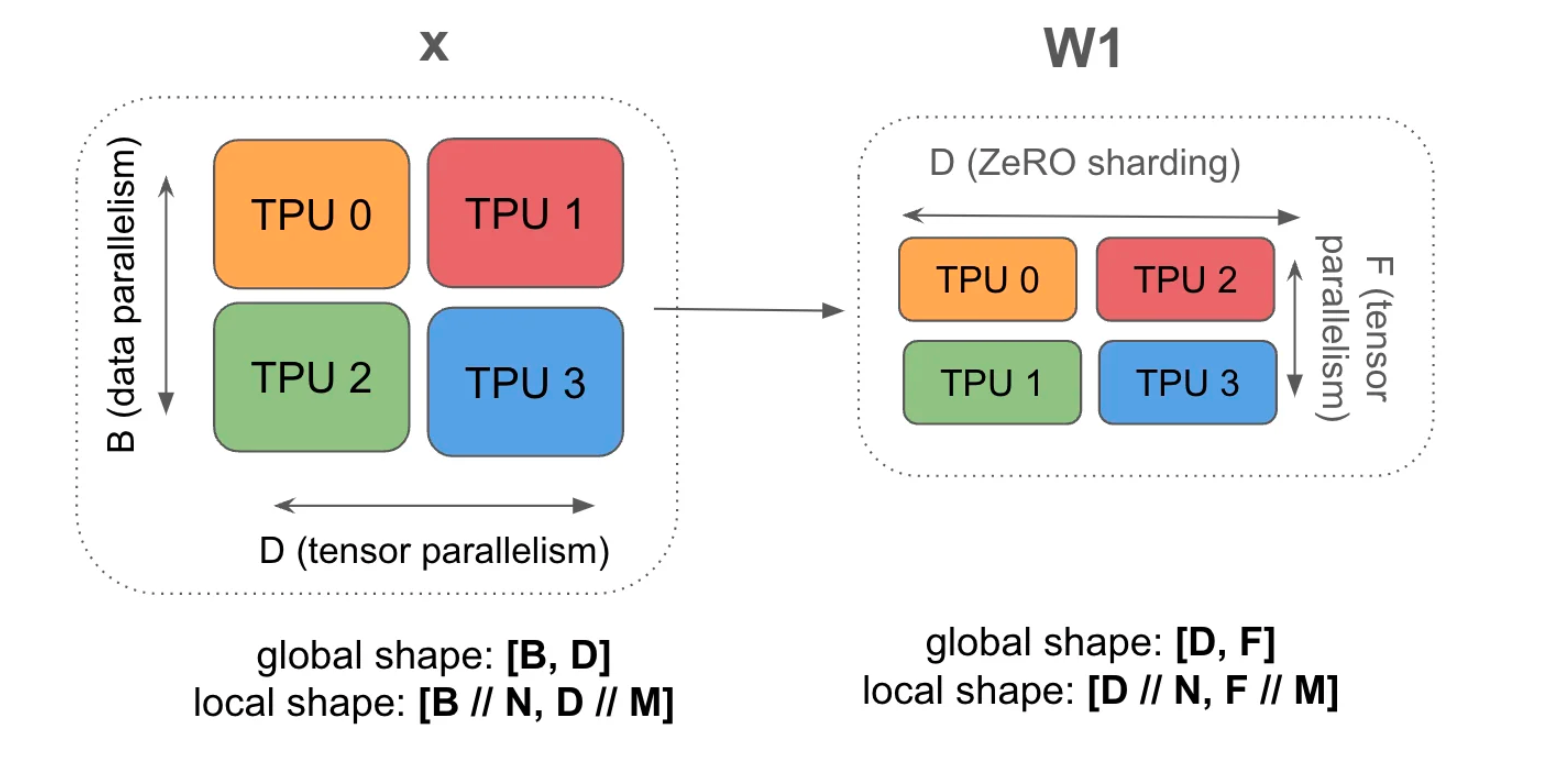
\includegraphics[width=0.5\linewidth]{fig/tensor.png}
    \caption{Tensor parallelism by sharding over both $X$ and $Y$ dimensions.}
\end{figure}

%----------- 导言区 ------------
%----------- 正文 --------------
\begin{tcolorbox}[
    title={Tensor Parallelism (Forward \& Backward)},
    colback=gray!6,
    colframe=black!70,
    boxrule=0.4pt,
    arc=2pt,
    left=4pt,right=4pt,top=4pt,bottom=4pt,
    label={fig:tensor_parallelism_algo},
    fontupper=\footnotesize\ttfamily,   % \small 亦可；等宽字体更像代码
    breakable
]

\textbf{Forward pass (compute Loss[$B_X$])}\\
In[$B_X,D$]         = AllGather\_Y(In[$B_X,D_Y$]) \textit{(critical)}\\
W\_in[$D,F_Y$]      = AllGather\_X(W\_in[$D_X,F_Y$]) \textit{(prefetch)}\\
Tmp[$B_X,F_Y$]      = In[$B_X,D$] ·\textsubscript{D} W\_in[$D,F_Y$]\\
W\_out[$F_Y,D$]     = AllGather\_X(W\_out[$F_Y,D_X$]) \textit{(prefetch)}\\
Out[$B_X,D$]\{U\_Y\}= Tmp[$B_X,F_Y$] ·\textsubscript{F} W\_out[$F_Y,D$]\\
Out[$B_X,D_Y$]      = ReduceScatter\_Y(Out[$B_X,D$]\{U\_Y\}) \textit{(critical)}\\
Loss[$B_X$]         = \dots\\

\vspace{0.4em}\tcbline\vspace{0.4em}  % 分隔线，可调整间距

\textbf{Backward pass (d$W_{\!out}[F_Y,D_X]$, d$W_{\!in}[D_X,F_Y]$)}\\
dOut[$B_X,D$]         = AllGather\_Y(dOut[$B_X,D_Y$]) \textit{(critical)}\\
dW\_out[$F_Y,D$]\{U\_X\} = Tmp[$B_X,F_Y$] ·\textsubscript{B} dOut[$B_X,D$]\\
dW\_out[$F_Y,D_X$]    = ReduceScatter\_X(dW\_out[$F_Y,D$]\{U\_X\})\\
W\_out[$F_Y,D$]       = AllGather\_X(W\_out[$F_Y,D_X$]) \textit{(prefetch)}\\
dTmp[$B_X,F_Y$]       = dOut[$B_X,D$] ·\textsubscript{D} W\_out[$F_Y,D$]\\
In[$B_X,D$]           = AllGather\_Y(In[$B_X,D_Y$]) \textit{(shared)}\\
dW\_in[$D,F_Y$]\{U\_X\}= dTmp[$B_X,F_Y$] ·\textsubscript{B} In[$B_X,D$]\\
dW\_in[$D_X,F_Y$]     = ReduceScatter\_X(dW\_in[$D,F_Y$]\{U\_X\})\\
W\_in[$D,F_Y$]        = AllGather\_X(W\_in[$D_X,F_Y$]) \textit{(prefetch)}\\
dIn[$B_X,D$]\{U\_Y\}  = dTmp[$B_X,F_Y$] ·\textsubscript{F} W\_in[$D,F_Y$]\\
dIn[$B_X,D_Y$]        = ReduceScatter\_Y(dIn[$B_X,D$]\{U\_Y\}) \textit{(critical)}\\
\label{fig:tensor_parallelism_algo}
\end{tcolorbox}



% \begin{figure*}[t!]
%     \footnotesize
%     \textbf{Forward pass: need to compute Loss[$B_X$]}
%     \begin{algorithmic}[1]
%         \STATE $\mathrm{In}[B_X, D] = \mathrm{AllGather}_Y(\mathrm{In}[B_X, D_Y])$ $ (\text{on critical path}) $
%         \STATE $W_\mathrm{in}[D, F_Y] = \mathrm{AllGather}_X(W_\mathrm{in}[D_X, F_Y])$ $ (\text{can be done ahead of time}) $
%         \STATE $\mathrm{Tmp}[B_X, F_Y] = \mathrm{In}[B_X, D] \cdot_D W_\mathrm{in}[D, F_Y]$
%         \STATE $W_\mathrm{out}[F_Y, D] = \mathrm{AllGather}_X(W_\mathrm{out}[F_Y, D_X])$ $ (\text{can be done ahead of time}) $
%         \STATE $\mathrm{Out}[B_X, D] \{U_Y\} = \mathrm{Tmp}[B_X, F_Y] \cdot_F W_\mathrm{out}[F_Y, D]$
%         \STATE $\mathrm{Out}[B_X, D_Y] = \mathrm{ReduceScatter}_Y(\mathrm{Out}[B_X, D] \{U_Y\})$ $ (\text{on critical path}) $
%         \STATE $\mathrm{Loss}[B_X] = \dots$
%     \end{algorithmic}
%     \label{alg:forward_new}

%     \vspace{0.5cm} % Add some vertical space between the two blocks

%     \textbf{Backward pass: need to compute $\mathrm{d}W_\mathrm{out}[F_Y, D_X], \mathrm{d}W_\mathrm{in}[D_X, F_Y]$}
%     \begin{algorithmic}[1]
%         \STATE $\mathrm{dOut}[B_X, D_Y] = \dots$
%         \STATE $\mathrm{dOut}[B_X, D] = \mathrm{AllGather}_Y(\mathrm{dOut}[B_X, D_Y])$ $ (\text{on critical path}) $
%         \STATE $\mathrm{d}W_\mathrm{out}[F_Y, D] \{U_X\} = \mathrm{Tmp}[B_X, F_Y] \cdot_B \mathrm{dOut}[B_X, D]$
%         \STATE $\mathrm{d}W_\mathrm{out}[F_Y, D_X] = \mathrm{ReduceScatter}_X(\mathrm{d}W_\mathrm{out}[F_Y, D] \{U_X\})$
%         \STATE $W_\mathrm{out}[F_Y, D] = \mathrm{AllGather}_X(W_\mathrm{out}[F_Y, D_X])$ $ (\text{can be done ahead of time}) $
%         \STATE $\mathrm{dTmp}[B_X, F_Y] = \mathrm{dOut}[B_X, D] \cdot_D W_\mathrm{out}[F_Y, D]$ $ (\text{can throw away dOut[B, D] here}) $
%         \STATE $\mathrm{In}[B_X, D] = \mathrm{AllGather}_Y(\mathrm{In}[B_X, D_Y])$ $ (\text{not on critical path + this can be shared with (2) from the previous layer}) $
%         \STATE $\mathrm{d}W_\mathrm{in}[D, F_Y] \{U_X\} = \mathrm{dTmp}[B_X, F_Y] \cdot_B \mathrm{In}[B_X, D]$
%         \STATE $\mathrm{d}W_\mathrm{in}[D_X, F_Y] = \mathrm{ReduceScatter}_X(\mathrm{d}W_\mathrm{in}[D, F_Y] \{U_X\})$
%         \STATE $W_\mathrm{in}[D, F_Y] = \mathrm{AllGather}_X(W_\mathrm{in}[D_X, F_Y])$ $ (\text{can be done ahead of time}) $
%         \STATE $\mathrm{dIn}[B_X, D] \{U_Y\} = \mathrm{dTmp}[B_X, F_Y] \cdot_F W_\mathrm{in}[D, F_Y]$ $ (\text{needed for previous layers}) $
%         \STATE $\mathrm{dIn}[B_X, D_Y] = \mathrm{ReduceScatter}_Y(\mathrm{dIn}[B_X, D] \{U_Y\})$ $ (\text{on critical path}) $
%     \end{algorithmic}
%     \label{alg:backward_new}

%     \caption{Pseudo-code for tensor parallelism along both $X$ and $Y$ dimensions.}
%     \label{fig:tensor_parallelism_algo}
% \end{figure*}

To address the issue with pure data parallelism, we consider tensor parallelism, which shards weights over devices. Sharding weights over the $X$ axis is sometimes referred tot as fully-sharded data parallelism (FSDP), and sharding over the $Y$ axis is sometime simply called tensor parallelism \cite[Part 5]{scaling-book}. However, we focus on sharding over both the $X$ and $Y$ axis, since sharding over only one axis will not be helpful in reducing the communication cost of each AllGather/ReduceScatter operation. This is due to, for example, when sharding a tensor of size $IJ$ over $n$ nodes in just the $X$ axis, the amount of data send/received by each node is still $\frac{m - 1}{m} IJ$.

Let $m_{i, X}$ and $m_{i, Y}$ be the number of nodes in the $i$-th cluster along the $X-$ and $Y-$axis of sharding, respectively, such that $m_{i, X} m_{i, Y} = m_i$. Let $p_{i, (j_X, j_Y)}$ be the relative size of the tensor shard assigned to node $(j_X, j_Y)$ in the $i$-th cluster, such that $\sum_{j_X} \sum_{j_Y} p_{i, (j_X, j_Y)} = 1$.

Our analysis refers to the pseudo-code in \textit{Tensor Parallelism (Forward \& Backward)} \ref{fig:tensor_parallelism_algo}. The formula for the the communication time costs are complicated. For example, the time it takes to perform $\mathrm{AllGather}_Y([B_X, D_Y])$ is
\begin{align*}
    \max_{0 \le j_X < m_{i, X}} \left\{\max \left\{\max_{0\le j_Y < m_{i, Y}} \left\{v_{i, (j_X, j_Y), (u)} + \frac{p_{i, (j_X, j_Y)} BD}{w_{i, (j_X, j_Y), (u)}} \right\}, \right. \right. \\
    \left. \left. max_{0\le j_Y < m_{i, Y}} \left\{v_{i, (j_X, j_Y), (d)}+ \frac{\sum_{j_Y' \ne j_Y} p_{i, (j_X, j_Y')} BD}{w_{i, (j_X, j_Y), (d)}} \right\} \right\} \right\}.
\end{align*}

To simplify our analysis, we approximate the communication  cost along the $Y$-axis with
\begin{align}
    v + \frac{BD}{\min m_{i, X} w},
\end{align}
which assumes uniform latency of $v$ and bandwidth of $w$. The communication cost along the $X$-axis can also be approximated with
\begin{align}
    v + \frac{FD}{\min m_{i, Y} w}.
\end{align}
It can be observed that the overall communication cost is reduced. However, the communication cost, on the other hand, is increased by
\begin{align}
    2\left(v + \frac{BD}{\min m_{i, X} w}\right)
\end{align}
on top the original communication cost of data parallelism. Therefore, applying tensor parallelism would be beneficial when $BD$ is small.

\section{Evaluation}
\begin{figure}[htbp]
    \centering
    \begin{minipage}[t]{0.3\textwidth}
        \centering
        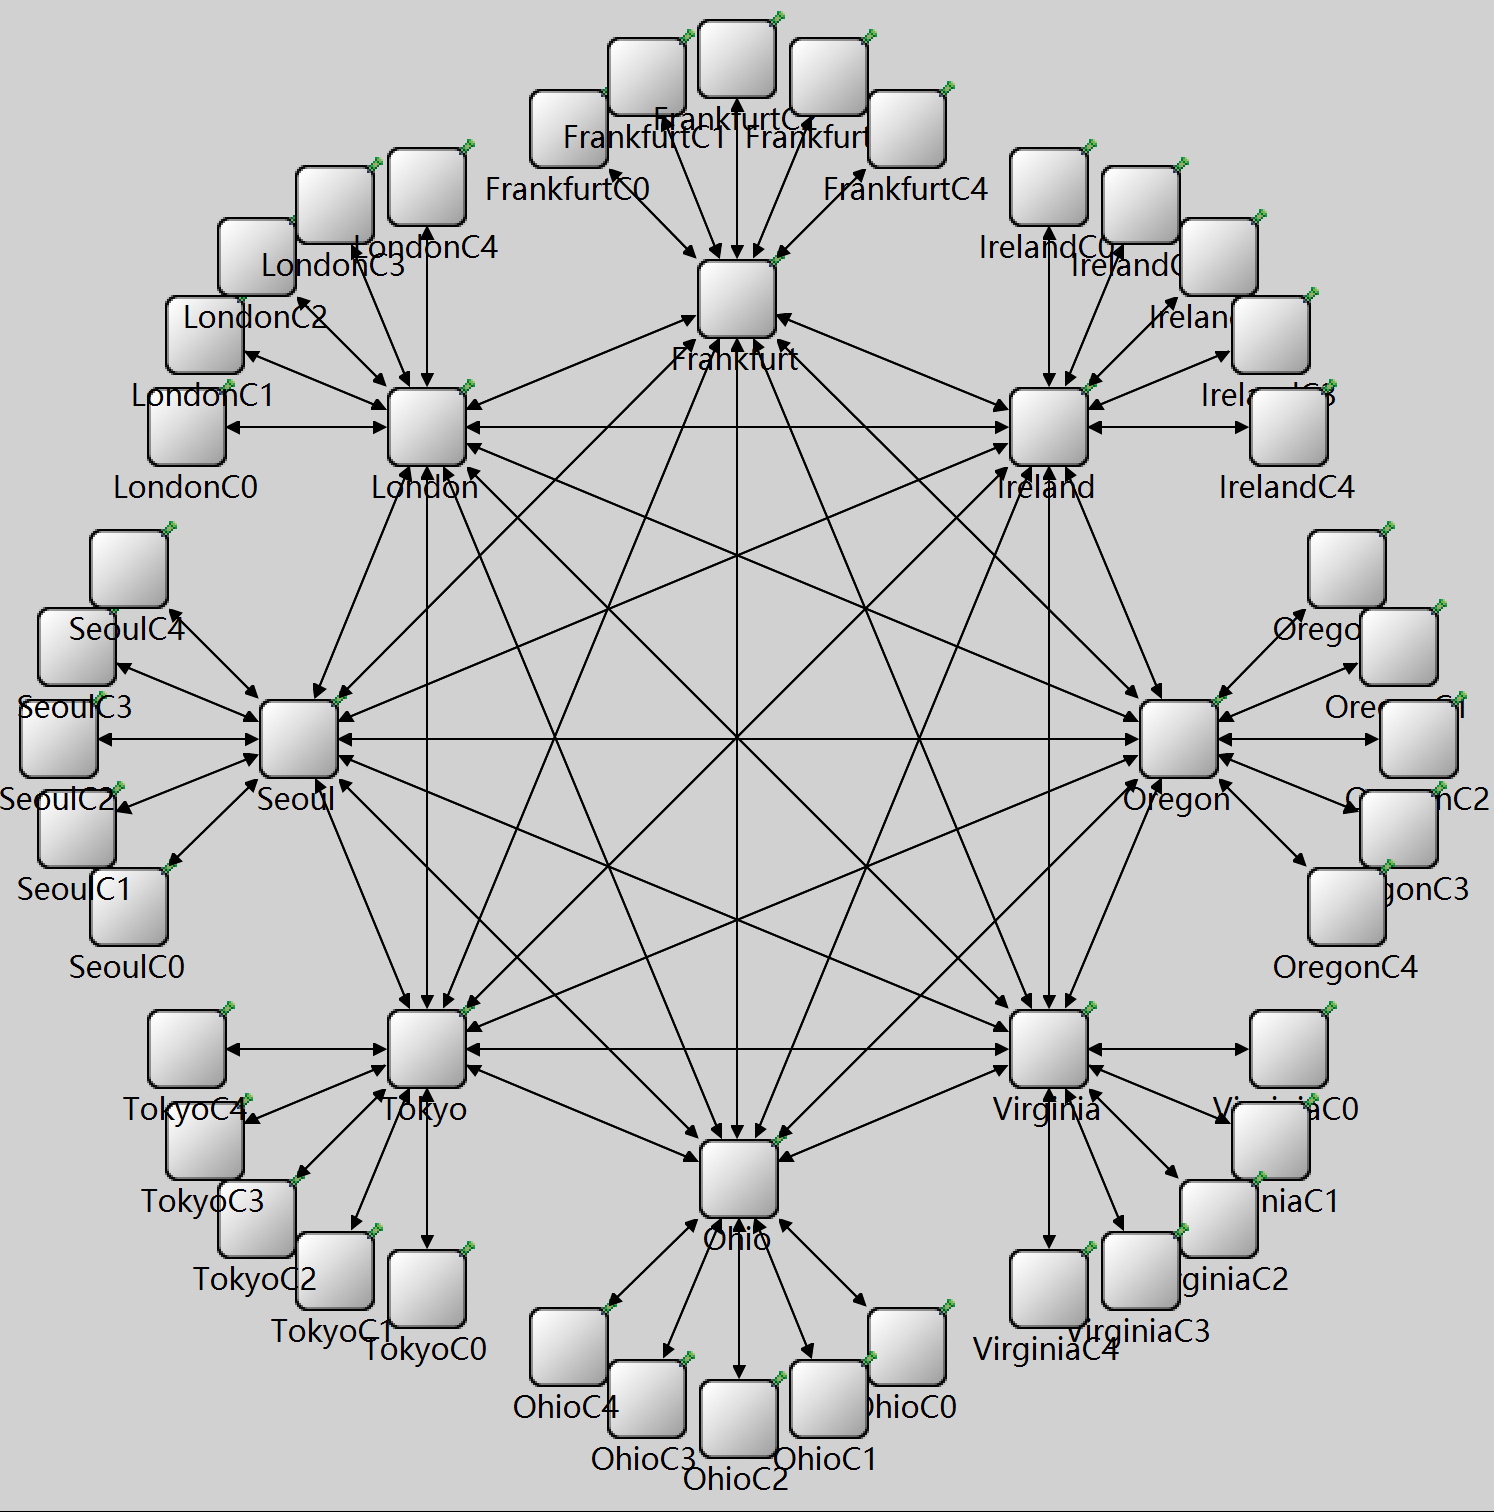
\includegraphics[width=0.95\linewidth]{fig/our_topology.png}
        \caption{The topology used in simulation with clusters located in Ohio, Virginia, Oregon, Ireland, Frankfurt, London, Seoul, and Tokyo AWS regions.}
        \label{fig:our_topology}
    \end{minipage}%
    \hfill
    \begin{minipage}[t]{0.68\textwidth}
        \centering
        \begin{tabular}{l|l}
            \hline
            \textbf{Parameter} & \textbf{Value} \\
            \hline
            $L$ (\# layers in the model) &  $126$ \\
            \hline
            $D$ (hidden dimension) & $16384$ \\
            \hline
            $F$ (feed-forward dimension) & $53248$ \\
            \hline
            $\mathcal{N}$ (\# input tokens) & $10^9$ \\
            \hline
            $\mathcal{B}$ (batch size) & $10^6$ \\
            \hline
            $n$ (\# clusters) & 8 \\
            \hline
            $m_i$ (\# clients in clusters) & 5 \\
            \hline
            $v_{i, j}, w_{i, j}$ & (median consumer link in country) \\
            \hline
            $V_{i, j}, W_{i, j}$ & (AWS instance benchmark) \\
            \hline
        \end{tabular}
        \caption{The parameters used in the simulation.}
        \label{tab:simulation_parameters}
    \end{minipage}
\end{figure}


\begin{figure}
    \centering
    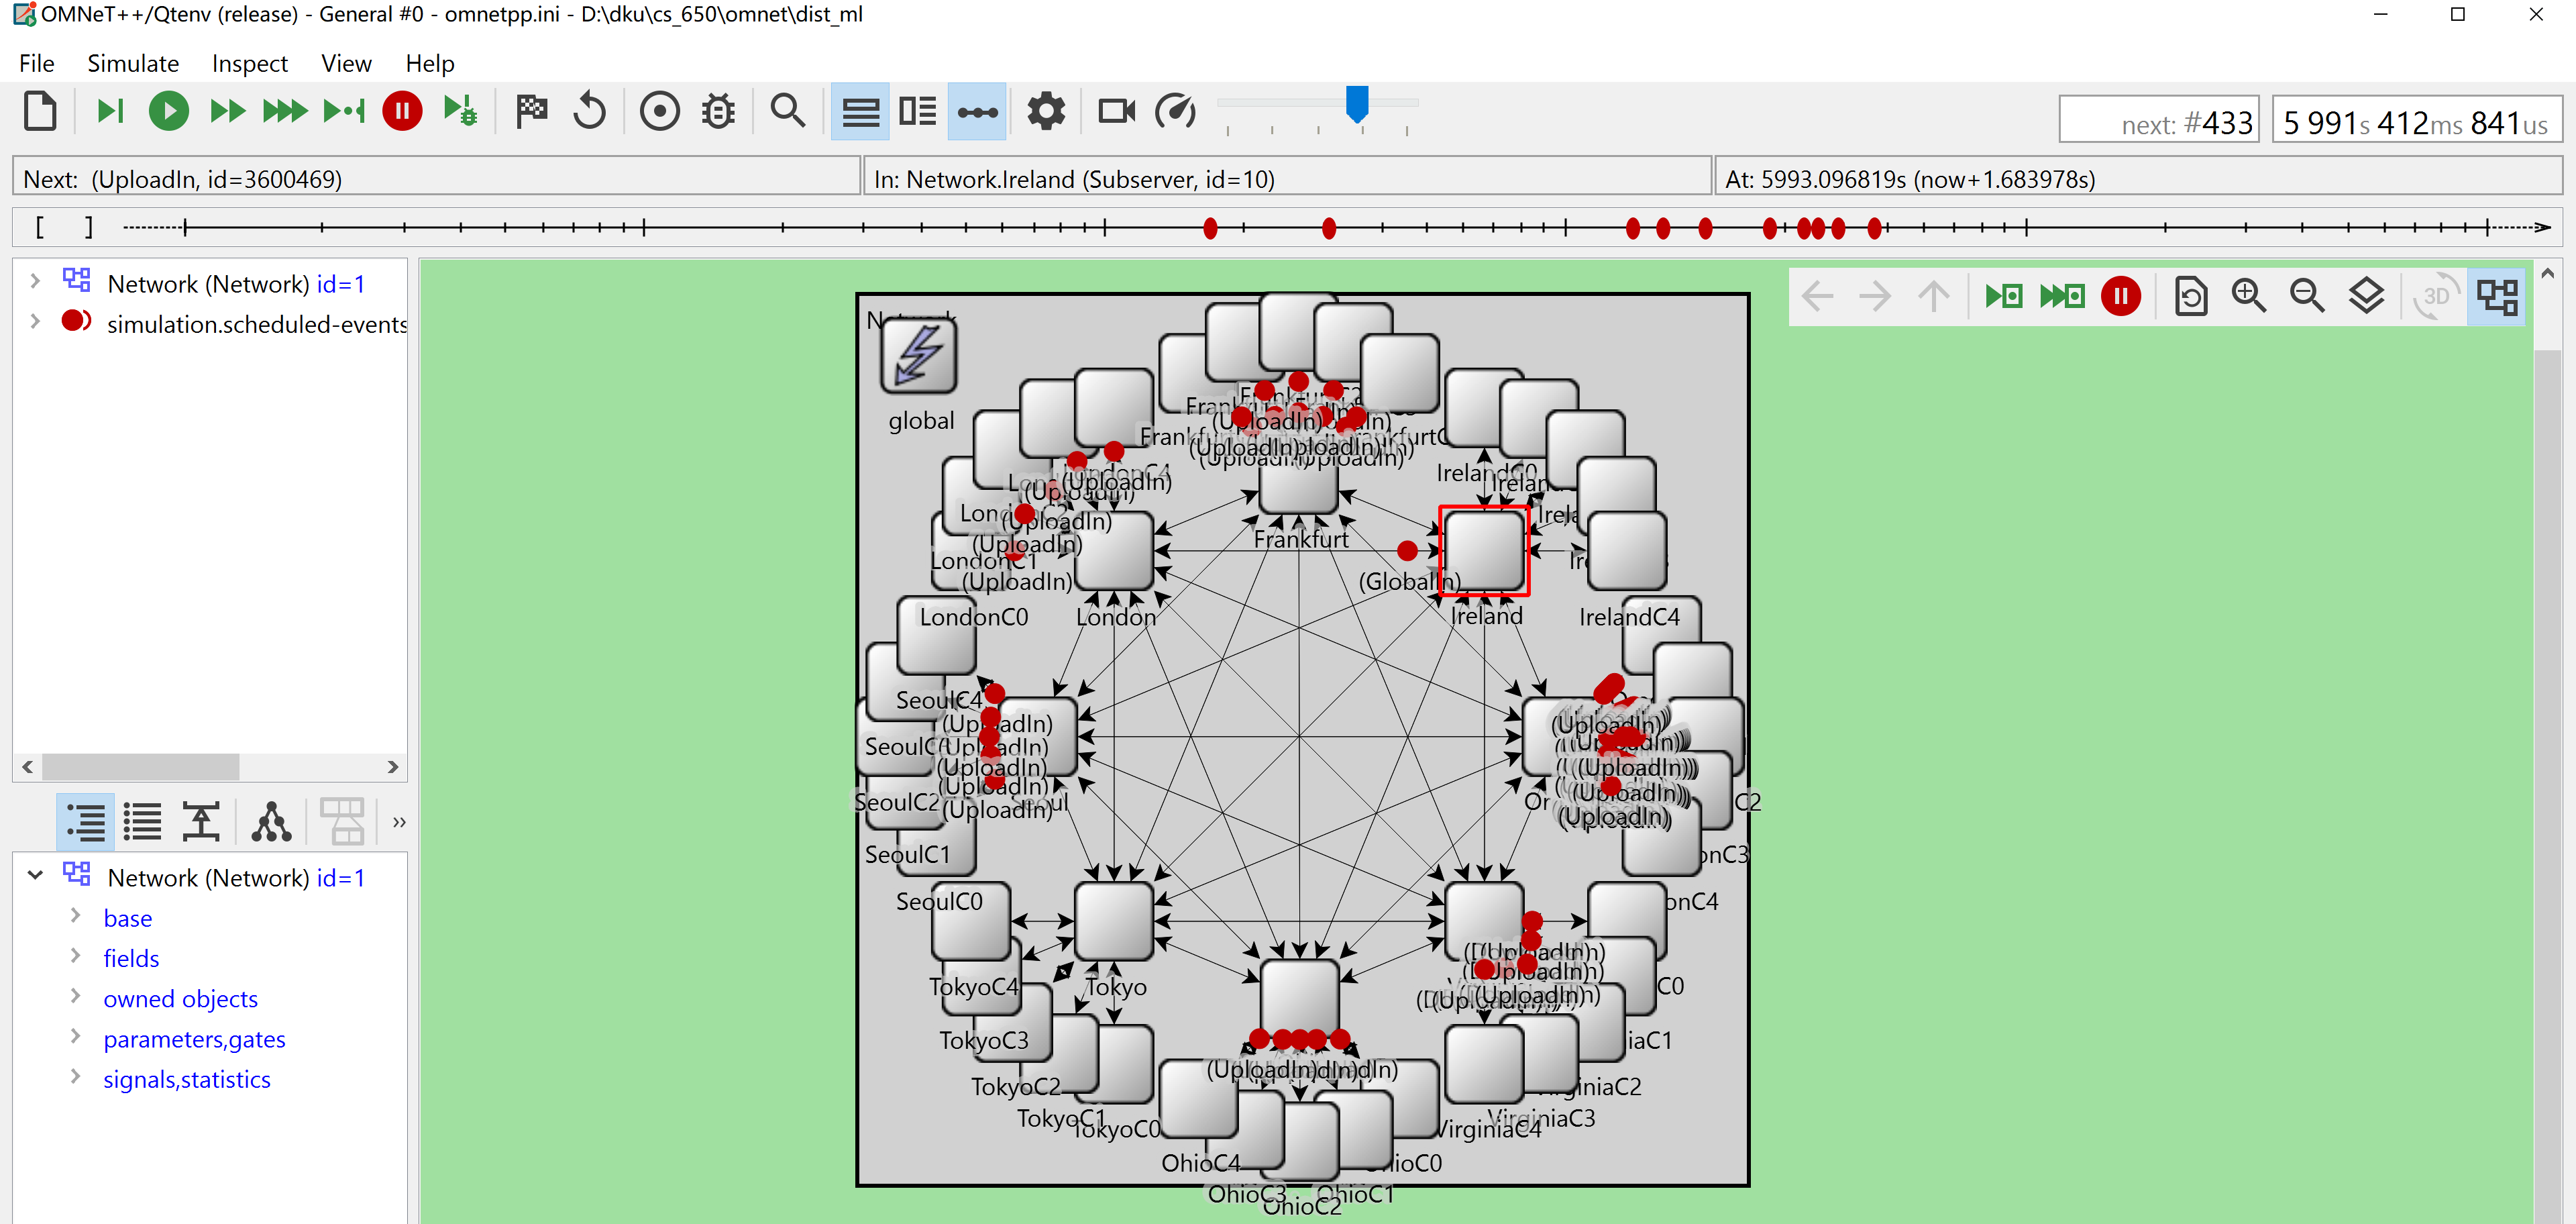
\includegraphics[width=0.9\linewidth]{simulation.png}
    \caption{Simulation in progress.}
    \label{fig:simulation}
\end{figure}


We use OMNeT++ \cite{opensim2001omnet}, a modular, component-based C++ simulation library and framework, to measure the simulated training time on a representative network \footnote{Code available at \url{https://github.com/theta-lin/cs-650-project-code}.}.

As shown in Figure \ref{fig:our_topology}, The representative framework consists of eight geo-distributed clusters with one subserver and five clients per cluster. We use the network latency and bandwidth between eight AWS instances distributed in eight AWS regions \cite[Sec. D.3]{yuan2022decentralized} for the inter-cluster latency and bandwidth. As for the intra-cluster latency and bandwidth, we use the median fixed broadband latency and bandwidth from Speedtest Global Index \cite{ookla2025speedtest} in the country where the AWS region of the corresponding subserver is located, which is representative of the consumer Internet link characteristics in different countries.

The parameters used in the simulation is shown in Table \ref{tab:simulation_parameters}. For the parameter sizes of the model being trained, we use the parameter sizes of Llama 3.1 405B \cite{meta2025llama}, which is representative of a large model that may require distributed training.

The strategy simulated in the experiment consists of pipeline parallelism between clusters and data parallelism within clusters. For simplicity, model layers are evenly distributed among clusters ($\frac{L}{n}$ layers per cluster), and input tokens are also evenly distributed among clients within clusters ($\frac{B}{m_i}$ tokens per client). Note that this simplification disregards the possible heterogeneity of total memory between clusters and did not adapt for the heterogeneity of the compute power between clients. The heterogeneity of inter-cluster link characteristics is exploited by enumerating all the permutations of the subservers and search for the permutation with the least total inter-cluster communication time before the simulation.

FLOPS utilization is used as a metric for the efficiency of the communication scheme. It can be calculated with:
\begin{align}
    \text{FLOPS utilization} = \text{actual FLOPS} \cdot \frac{1}{\text{total client FLOPS}} = \frac{4 \cdot \mathcal{N}DFL}{T_{\text{actual}}} \frac{1}{\sum_{i=0}^{n-1} \sum_{j=0}^{m_i-1} c_{i, j}}
\end{align}

\begin{figure}
    \centering
    \small
    \begin{tabular}{l|l|l}
        \hline
        \textbf{$B$ (micro-batch size)} & \textbf{Time to train ($T_{\text{actual}}$ in days)} & \textbf{FLOPS utilization} \\
        \hline
        $100,000$ & $581.36$ & $2.43 \times 10^{-4}$ \\
        \hline
        $50,000$ & $476.70$ & $2.97 \times 10^{-4}$ \\
        \hline
        $10,000$ & $452.70$ & $3.12 \times 10^{-4}$ \\
        \hline
    \end{tabular}
    \caption{Simulation result with fixed client FLOPS $c_{i, j} = 3 \times 10^{14} j$ and varying micro-batch size $B$.}
    \label{tab:simulation_micro_batch}
\end{figure}

We first investigate the impact of micro-batch size on training performance. For simplicity, the client FLOPS's are set to $c_{i, j} = 3 \times 10^{14} (j + 1)$ across all clusters. This is to roughly match NVIDIA A100 80GB PCIe Tensor Core's $3.12 \times 10^{14}$ FLOPS BFLOAT16 compute performance \cite{nvidia2020a100}. The results are shown in Table \ref{tab:simulation_micro_batch}. Note that FLOPS utilization is very low, indicating that the training speed is bottlenecked by the network communication cost.

%\textbf{TODO: need citation on batch size and training time}

\begin{figure}
    \centering
    \small
    \small
    \begin{tabular}{l|l|l}
        \hline
        \textbf{$c_{i, j}$ (client FLOPS)} & \textbf{Time to train ($T_{\text{actual}}$ in days)} & \textbf{FLOPS utilization} \\
        \hline
        $3 \times 10^{12} (j + 1)$ & $483.35$ & $2.92 \times 10^{-2}$ \\
        \hline
        $3 \times 10^{13} (j + 1)$ & $477.22$ & $2.96 \times 10^{-3}$ \\
        \hline
        $3 \times 10^{14} (j + 1)$ & $476.70$ & $2.97 \times 10^{-4}$ \\
        \hline
    \end{tabular}
    \caption{Simulation result with fixed micro-batch size $B=50,000$ and varying client FLOPS $c_{i, j}$.}
    \label{tab:simulation_flops}
\end{figure}

To further investigate the impact of network communication on training performance, we fix micro-batch size to $B = 50,000$ and varies the client FLOPS. Results in Table \ref{tab:simulation_flops} indicates that the FLOPS utilization indeed improves as client FLOPS decreases. This indicates that in our representative network topology, the training time is highly dominated by the network communication time. Therefore, such a distributed training scheme might not be feasible in the current Internet infrastructure.


\section{Related Work}\label{sec:related}

\paragraph{Multi‑dimensional parallelism.}
Early systems such as GPipe introduced inter‑batch \emph{pipeline parallelism} to hide WAN‑scale latencies for very deep models~\cite{huang2019gpipe}.  
PipeDream generalised this idea with weight stashing and micro‑batching, achieving up to $5.3\times$ speed‑ups over pure data parallelism \cite{narayanan2019pipedream}. 
On the intra‑layer axis, Megatron‑LM pioneered coarse‐grained \emph{tensor parallelism} that shards each matrix across multiple GPUs while keeping communication local \cite{shoeybi2019megatron}.  
Our work not only combines these dimensions, but crucially adds a third geo‑hierarchical tier (the subserver) that was absent from earlier designs.

\paragraph{Geo‑distributed training.}

\cite{yuan2022decentralized} introduces geo-distributed machine learning for large language models. However, they haven't consider subserver or tensor parallelism analysis. Recent methods such as NetStorm dynamically reshaping spanning‑tree topologies to match fluctuating WAN links and achieves $6.5$–$9.2\times$ faster synchronisation \cite{li2024accelerating}.  
Our subserver abstraction can be viewed as a pragmatic middle ground: it retains synchronous SGD, but limits long distance transfers to a single per‑step pipeline message.


\smallskip
In summary, prior work either optimises one parallel dimension, assumes uniform fabrics, or targets asynchronous geo‑ML.  
We instead provide the first end‑to‑end analysis of \emph{heterogeneous, synchronous} training that spans metropolitan clusters via subservers.

\section{Conclusion \& Future Work}\label{sec:conclusion}

We introduced a \emph{subserver‑centred} architecture that bridges metro‑scale GPU with long‑haul optical links and analysed how to layer pipeline, data and tensor parallelism on top of this two‑tier network.  Moreover, we also conducted simulation on OMNeT++ with eight AWS regions and clusters across these regions to calculate training time, FLOPS utilization.


The next step could be deploying the full stack on a real multi‑region testbed and train a 7‑to‑70 B‑parameter Transformer to quantify convergence, energy and cost trade‑offs. We believe these steps will move geo‑distributed training from simulation to a deployable reality, unlocking the computational headroom required for \SI{100}{T}‑scale frontier models.


% \item \textbf{Communication-Topology Optimization.} We will design and implement collective communication routines (e.g., AllReduce, AllGather) that adapt to heterogeneous network topologies. By analyzing link bandwidths and latency characteristics, we aim to minimize data-transfer bottlenecks during gradient aggregation.

% \bibliographystyle{IEEEtran}

\section*{ML Tool Use}

ML tools including ChatGPT-4o and NotebookLM have been used for researching and summarizing text and to refine and improve the grammar and format of the text and pseudo code.

\printbibliography


\end{document}